\documentclass[conference]{IEEEtran}
\IEEEoverridecommandlockouts
% The preceding line is only needed to identify funding in the first footnote. If that is unneeded, please comment it out.
\usepackage{amsmath,amssymb,amsfonts,mathtools}
\usepackage{hyperref}
\usepackage{cleveref}
\usepackage{algorithmic}
\usepackage{graphicx}
\usepackage{booktabs}
\usepackage{tikz}
\usepackage{pgf}
\usepackage{textcomp}
\usepackage{xcolor}
\usepackage{float}
\usepackage[sorting=nyt, style=numeric, backend=biber]{biblatex}
\usepackage{caption}
\usepackage{subcaption}
\addbibresource{bibliography.bib}
\def\BibTeX{{\rm B\kern-.05em{\sc i\kern-.025em b}\kern-.08em
    T\kern-.1667em\lower.7ex\hbox{E}\kern-.125emX}}
\DeclarePairedDelimiter{\abs}{\lvert}{\rvert}	%Absolute value


% Information for generating title
\title{U-Net for segmenting fascicles in vagus nerve histologies}

\author{
\IEEEauthorblockN{Bioli Ivan}
\IEEEauthorblockA{\href{mailto:ivan.bioli@epfl.ch}{ivan.bioli@epfl.ch}}
\and
\IEEEauthorblockN{Cao Khanh Nguyen}
\IEEEauthorblockA{\href{mailto:cao.nguyen@epfl.ch}{cao.nguyen@epfl.ch}}
\and
\IEEEauthorblockN{Hasan Syed Umer}
\IEEEauthorblockA{\href{mailto:umer.hasan@epfl.ch}{umer.hasan@epfl.ch}}}

\begin{document}

\maketitle
    \begin{abstract}
   A model for automating the segmentation of fascicles in vagus nerve histologies has been implemented by using a U-Net-based architecture. We apply data augmentation and test different loss functions to address the problem of highly imbalanced classes. Finally, we apply post-processing techniques to improve the model performance.   
    \end{abstract}


\section{Introduction}
\label{sec:introduction}
The vagus nerve (VN) is the largest nerve in the autonomic nervous system; it innervates most truncal organs, including heart, lungs, stomach, and intestines, and is responsible for various internal organ functions, such as heart rate control, digestion, and immune response \cite{vagus}. The VN is surgically accessible at some points along its path and VN Stimulation (VNS) \cite{vns} proved to be effective in the treatment of epilepsy \cite{epilepsy}, rheumatoid arthritis \cite{arthritis}, and other serious diseases. Nonetheless, state-of-the-art VNS is still not selective enough and causes non-negligible side effects. The fibres constituting peripheral nerves are organised into bundles called fascicles, which are electrically insulated from the surrounding tissue. Thus, understanding the fascicular organisation in the VN can help deliver selective VNS. Such information can be obtained by analysing histological stained sections of the target nerve, after that fascicles are singled out from other nerve tissues. This process is called segmentation, and performing it manually on large datasets is impractical. 

The present work focuses on the implementation of machine learning techniques to segment fascicles in VN histologies. We apply semantic segmentation using an instance of the U-Net convolutional neural network family \cite{unet} to solve the described problem. 


\section{Methods}
\subsection{Dataset}
Our dataset consists of 924 VN histologies, out of which 85 are provided with manually annotated ground-truth masks (segmented masks). We visually inspected the dataset and discarded 51 images, including 13 of the ones with ground truth masks. Of the 72 remaining segmented masks, 63 have been used for training, while 9 have been used for validation. Both images and masks are downsampled to 512 x 512 pixels. Images are RGB-coded in (0, 1) (three channels), while masks are binary (one channel).
\subsection{Data augmentation}
We performed data augmentation by applying to each (image, mask) couple proposed during training one random complex transformation, which is obtained by composing the following elementary transformations:
\begin{itemize}
    \itemsep0em
    \item Random image rotations between 0 and 359 degrees.
    \item Random translations in the x and y direction with the magnitude of the shift being a maximum of 20\% of the respective image dimension.
    \item Random shear between 0 and 30 degrees.
    \item Random image scaling in the x and y directions from 0.9 to 1.1.
\end{itemize}
The final transformation for each sample was, thus, an affine transformation.
As histologies may also vary in colour and brightness, we added to the aforementioned geometrical transformation a “colour” transformation, consisting of random channel shifts (with a maximum shift of 20\%) and random brightness shifts (ranging from 60\% to 140\% brightness).

Finally, we visually inspected the augmented images to check the validity of the above listed transformations.

\subsection{Model architecture}
For our segmentation network, we follow the U-Net architecture \cite{unet}. We chose this widely used architecture since its proposers have shown that it provides good predictions even using a relatively small training dataset if data augmentation techniques are correctly applied. The original U-Net consists of the down-sampling of inputs and the up-sampling steps, forming a U-shape. The network includes five blocks of fully connected convolutional layers, combined with “ReLU” activation, 2x2 max-pooling layers, and batch normalisation for the down-sampling part. In the up-sampling part, the outputs of the first half are fed to fully connected transposed convolutional layers. Finally, the output of the second half is fed into a linear layer to classify each pixel.
 
Furthermore, our architecture slightly adapts the original U-Net provided in \cite{unet}. The architecture from the original paper applies skip connections to transfer the information on locations from the down-sampling to the up-sampling half. In our model, we removed those connections and used XCeption-like residual connections instead \cite{xception}. The output of each block is saved as residual and added to the output of the following block, such as depicted in \Cref{fig:unet}. The purpose of this extra step is to reduce the computational costs of fully convolutional networks. The patching of each block with the immediate residual from the previous one would also help retaining and propagating relevant information about the location and semantic structures of the pixels. This approach is inspired by the tutorial on U-Net based image segmentation \cite{unet_keras}. All implementations are developed in the Keras framework.

\begin{figure}[ht]
\centering
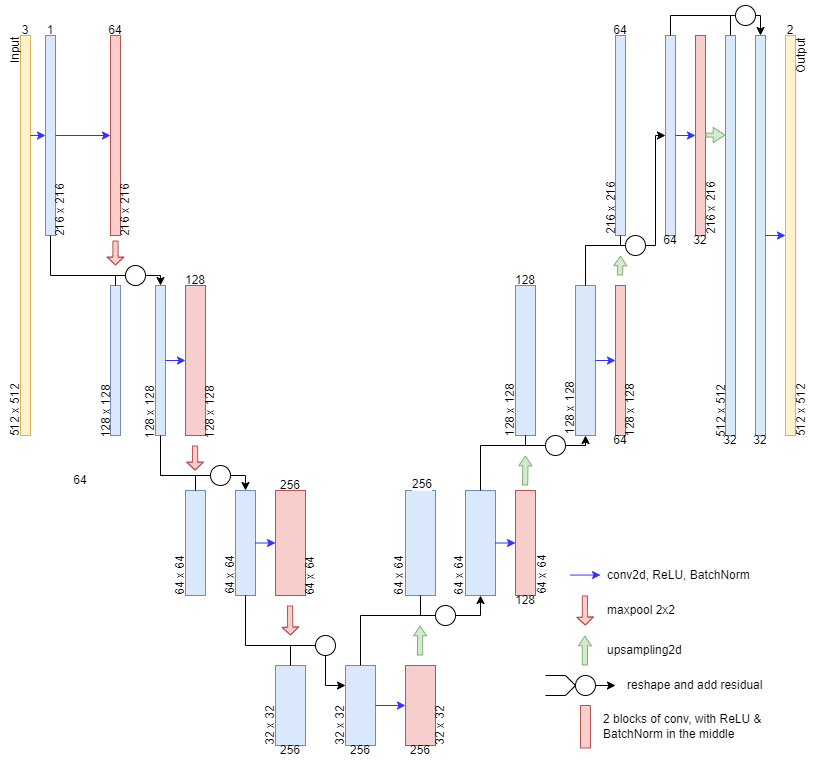
\includegraphics[width=0.7\columnwidth]{figures/U-Net-XCeption.png}
\caption{Visual description of the U-Net with XCeption-like residual connections.}
\label{fig:unet}
\end{figure}

\subsection{Loss functions and evaluation metrics}
To train the network, we use 3 different loss functions and compare the performances of the obtained models. For each pixel, let us indicate with $y$ the ground truth mask value (i.e. $y=1$ for fascicle, $y=0$ for background), and with $p$ the probability of being classified as a fascicle pixel. In addition, let $p_t = py+(1-p)(1-y)$. The first loss function used is the Binary Cross Entropy (BCE) loss, which is the loss recommended in the original U-Net paper \cite{unet}. At pixel level, the BCE loss is defined as $-(y\log(p)+(1-y)\log(1-p))=-\log(p_t)$. The overall BCE loss is the average value of BCE computed over all the pixels. 

The BCE loss equally penalises false positives and false negatives, thus, if the two classes are strongly imbalanced, this loss is prone to favour the most frequently represented class. In our dataset, the average ratio between the area of the fascicles and the background area in the Training Set (TS) is equal to 0.154. Therefore, the Focal Loss (FL) \cite{focal_loss} is used to down-weight "easy" correct classifications and focus on "hard" negative classifications. For each pixel, FL is defined as $-\alpha_t(1-p_t)^{\gamma}\log(p_t)$, i.e. a modulating factor $\alpha_t(1-p_t)^{\gamma}$ is added to the BCE loss, where $\gamma$ and $\alpha_t$ are parameters of the loss. Misclassifications are associated with low values of $p_t$. Therefore, their contribution to the loss is almost unaffected, while the loss for correctly classified pixels is down-weighted. The higher $\gamma$, the higher the effect of the modulating factor. We train our model using FL, with parameters $\gamma = 2$ and $\alpha = 0.25$, as suggested in \cite{focal_loss}. 
We also train our model with a combination of BCE loss and FL, where both are weighted equally. We will refer to this loss as BCE+FL. 

To evaluate the performance of our model, we use two evaluation metrics: Intersection over Union (IoU) and Dice Loss (DL). Let us indicate with $GT$ the ground truth fascicles and let us define \emph{predicted fascicles} ($PF$) the connected components of the predicted foreground. Then IoU and DL are defined as 
\begin{equation*}
    \mathrm{IoU} = \frac{\abs{GT \cap PF}}{\abs{GT \cup PF}} \qquad
    \mathrm{DL} = 1 - \frac{\abs{GT \cap PM}}{\abs{GT} + \abs{PM}}
\end{equation*}

\subsection{Training}
The network is trained for 100 epochs using Adam with a learning rate of 0.01 as an optimizer. Due to the small number of histologies with available ground truth, using a high number of epochs might lead to overfitting. Therefore, we save the model at the epoch with the best validation loss.

\subsection{Post-processing}
As a first post-processing technique, we remove the predicted fascicles having an area lower than a predefined threshold value. Such threshold is set as the 0.01-quantile of the areas of all the fascicles present in the ground truth masks of the TS. In this way, we can be confident that the removed predicted fascicles are unlikely to be present in the histology. 
Moreover, different fascicles are sometimes merged already in the ground truth masks and, therefore, could also be merged by our model. To separate merged fascicles, we use the watershed algorithm \cite{watershed_article, watershed_tutorial}. 

Finally, we mark in red possibly merged or incorrectly predicted fascicles, i.e. fascicles with an area above the 0.99-quantile of the fascicles’ area in the TS and fascicles with an eccentricity above the 0.99-quantile of the fascicles’ eccentricity in the TS. 

\section{Results and Discussion}
\subsection{Training}
The use of the FL resulted in weighting too low the errors in classification of background, with random predictions dominated by the fascicle class. Trying different values of $\gamma$ and $\alpha_t$ was not effective. 
On the contrary, BCE loss and BCE+FL produced acceptable results. The plot of the metrics against the epochs during the training is shown in \Cref{fig:metrics}. In terms of the proposed evaluation metrics, the obtained models' results are summarised in \Cref{tab:result}. 

\begin{figure}[ht]
\makebox[\columnwidth][c]{
\begin{subfigure}{0.49\linewidth}
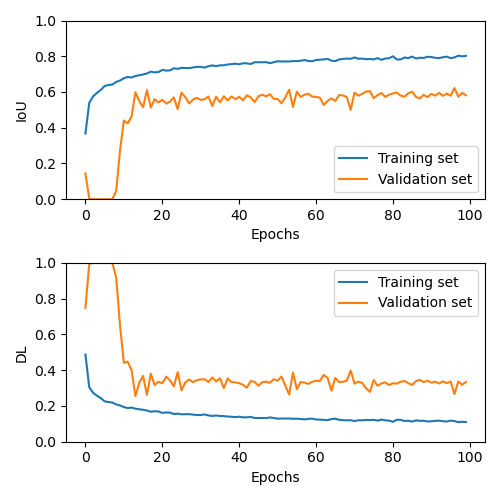
\includegraphics[width=\linewidth]{figures/training_metrics_BCE.png}
\caption{Training with BCE loss.}
\end{subfigure}\hspace*{\fill}
\begin{subfigure}{0.49\linewidth}
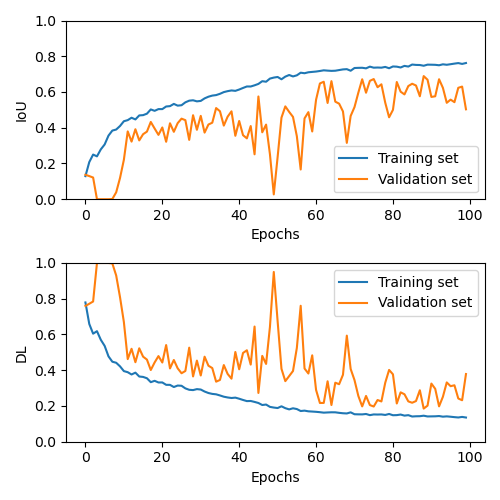
\includegraphics[width=\linewidth]{figures/training_metrics_FL+BCE.png}
\caption{Training with BCE+FL.}
\end{subfigure}\hspace*{\fill}}
\caption{Plots of the metrics against the epochs for the training with BCE loss and with BCE+FC.}
\label{fig:metrics}
\end{figure}

\begin{table}[h]
\caption{Average metrics over training (TS) and validation (VS) sets for the models trained with BCE loss and BCE+FL.}
\label{tab:result}
\centering
\begin{tabular}{lcccc}
 &\multicolumn{2}{c}{BCE} &\multicolumn{2}{c}{BCE+FL} \\
 & TS & VS & TS & VS \\
 \midrule
 IoU & 0.734 & 0.596 & 0.746 & 0.689 \\
 DL	& 0.153 & 0.287 & 0.145 & 0.185\\
 BCE & 0.088 & 0.136 & 0.446 & 0.462 \\
 FL	& 4.841	& 4.680	& 0.339	& 0.330 \\
 \bottomrule
\end{tabular}
\end{table}

Training with BCE loss, the best validation loss is attained at epoch 26. Noticeably, the IoU score on the validation set improves from 0 to above 0.5 in a low number of epochs remaining then almost constant for the rest of the training. This suggests that overfitting on the TS is occurring. Similar behaviour can be observed in the DL.

On the contrary, using an equally weighted combination of BCE loss and FL proved the best performance.  The best validation loss is obtained at epoch 89, resulting in the best validation IoU and DL among the three models. Interestingly, the IoU and the DL do not improve much on the TS, but they do on the validation set, i.e. we generalise better than using the BCE only. This is also confirmed by the fact that the IoU score and the DL keep improving almost along the whole training run, contrary to what happens when training with BCE loss. Furthermore, the value of the BCE loss attained training with BCE+FL is five times higher than the one obtained training with BCE only, but despite this, the IoU score and the FL are improved. This confirms that the BCE loss does not capture the semantic segmentation problem well when the two classes are highly imbalanced. \Cref{fig:validation} shows the predictions of the model trained with BCE+FL on three exemplar images from the validation set, compared with the ground truth. 

\begin{figure}[ht]
\centering
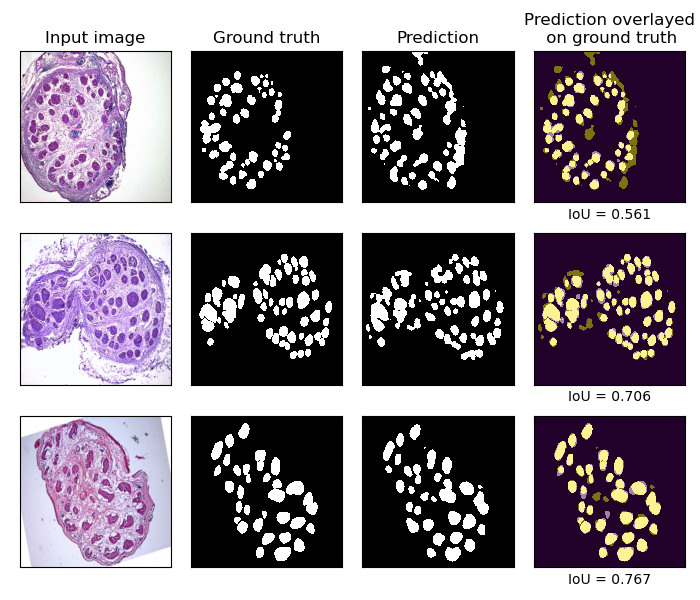
\includegraphics[width=\columnwidth]{figures/sample_predictions_wstats.png}
\caption{Predictions of the model trained with BCE+FL on three exemplar images from the validation set.}
\label{fig:validation}
\end{figure}

The predictions on 3 exemplar images from the unlabelled set are shown in \Cref{fig:unlabelled}. Noticeably, predictions on the third image are not accurate. The comparison between the colour histogram of the 3 images and the average colour histogram of the TS (see \Cref{fig:colour}) suggests a reason for this issue. The colour values of the third image are more concentrated, i.e. the image shows a lower contrast, which makes the fascicles identification more difficult. The colour transforms in the data augmentation were supposed to help us generalise to these images, but they proved not to be sufficient.

\begin{figure}[ht]
\centering
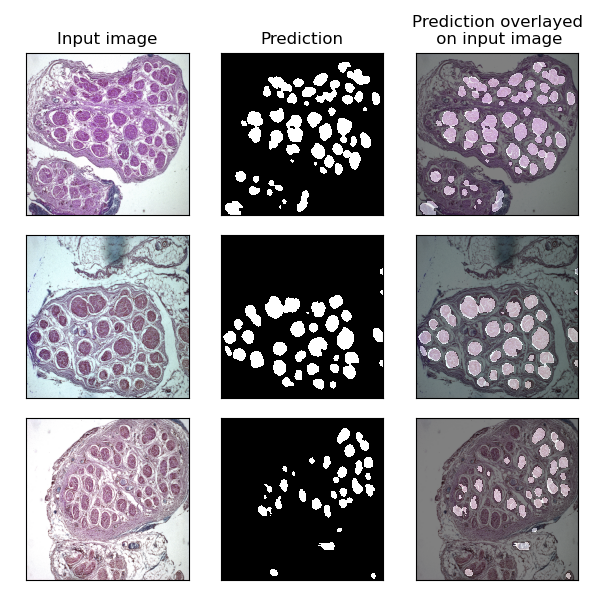
\includegraphics[width=\columnwidth]{figures/sample_predictions_unlabelled.png}
\caption{Predictions of the model trained with BCE+FL on three exemplar images from the unlabelled set.}
\label{fig:unlabelled}
\end{figure}
\begin{figure}[ht]
\centering
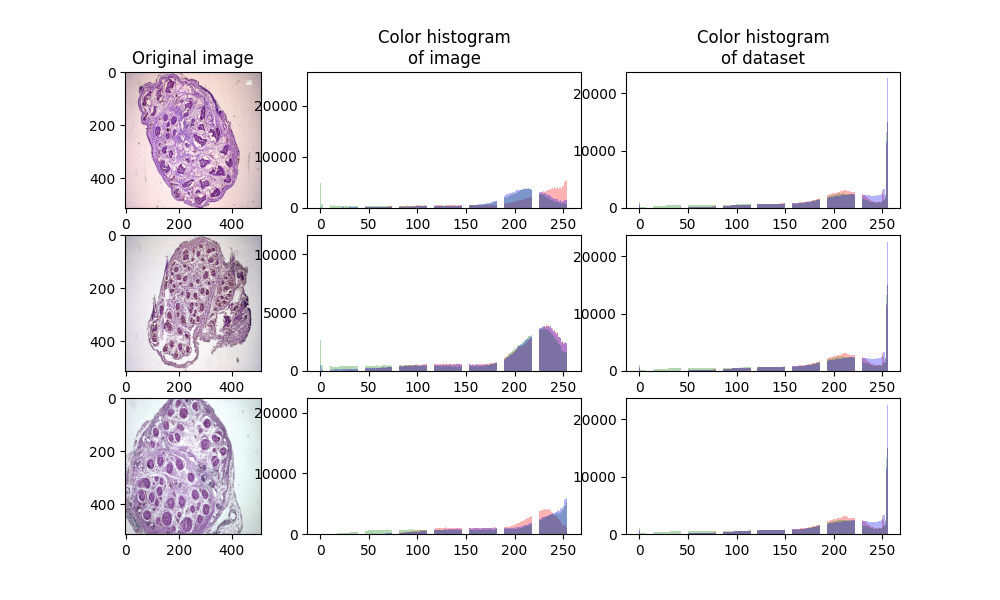
\includegraphics[width=\columnwidth]{figures/color_histograms.png}
\caption{Average colour histogram on the TS and colour histogram of three sample images from the unlabelled set for which the predictions are displayed.}
\label{fig:colour}
\end{figure}

\subsection{Post-processing}

\begin{figure}[]
\begin{subfigure}{1\linewidth}
\centering
\includegraphics[width=0.9\linewidth]{figures/distribution_before.png}
\caption{Before post-processing}
\label{fig:before}
\end{subfigure}
\begin{subfigure}{1\linewidth}
\centering
\includegraphics[width=0.9\linewidth]{figures/distribution_after.png}
\caption{After post-processing}
\label{fig:after}
\end{subfigure}
\caption{Histograms of fascicles areas, number and eccentricity before and after the post-processing.}
\label{fig:histograms}
\end{figure}

We then analyzed the distributions of the fascicles areas and eccentricity of the ground truth and of the predictions on the TS (see \Cref{fig:histograms}). It can be observed that our model predicts with a higher frequency than the effective one fascicles with small areas (i.e. artefacts) and with a very low or very high eccentricity, which might both be caused by merged fascicles or more in general incorrect predictions.

It should also be noticed that the issues of merging fascicles and predicting inexistent fascicles with small areas might also be caused by the loss functions used. Indeed, both BCE and FL are obtained as the average of pixel-wise losses. Therefore, they are not sensitive to boundary points of the fascicles, which are much less represented than interior points. Consequently, they do not heavily penalise the merging of different nearby fascicles in a single fascicle. Moreover, if the model predicts fascicles not present in the ground truth, they are not penalised too much if their area is small.

The proposed post-processing techniques partially solve the above mentioned issues. Indeed, it can be observed in \Cref{fig:after} that the histograms of the predicted fascicles areas, numbers and eccentricity values after post-processing are more similar to the ones computed using the ground truth masks. In particular, with respect to the histograms shown in \Cref{fig:before},  the peaks in the histogram of the areas corresponding to small area values are reduced, while the peaks corresponding to low and high eccentricity values are eliminated.

Post-processing effects on two images from the unlabelled set is shown in \Cref{fig:postprocessing}. It can be observed that fascicles with small areas are removed and that the use of the watershed algorithm effectively helps separating merged fascicles. Furthermore, one predicted fascicle is signalled as possibly merged, as it actually is. However, some predicted fascicles that are not separated nor coloured in red are still present even after the post-processing stage.
\begin{figure}
\centering
\includegraphics[width=\columnwidth]{figures/predictions_with_postprocessing_arrows.png}
\caption{Effects of post-processing on 2  images among the ones in Fig. 4. Merged fascicles separated by watershed algorithm are highlighted in red, removed predictions are in shown green.}
\label{fig:postprocessing}
\end{figure}


\section{Conclusions}
A U-Net based architecture for fascicles segmentation in VN histologies was developed. As loss functions, BCE, FL and BCE+FL were used to train the model, with the latter having the best performance in terms of IoU score. The model predictions were tested on unlabelled data, observing that the colour distribution can affect the model performance. Therefore, image pre-processing techniques could be applied, together with the addition of more colour transformations in the data augmentation. Moreover, loss functions penalising fascicles merging should be explored.

\newpage
\nocite{*}
\printbibliography
\end{document}
